\documentclass[12pt]{article}
\usepackage[top=1in, bottom=1in, left=1in, right=1in]{geometry}
\usepackage[justification=centering]{caption}
\usepackage{graphicx}
\usepackage{listings}
\usepackage{color}
\usepackage{indentfirst}
\usepackage{hyperref}

\lstset{ %
	%language=C,                % choose the language of the code
	basicstyle=\footnotesize,       % the size of the fonts that are used for the code
	                  % how far the line-numbers are from the code
	backgroundcolor=\color{white},  % choose the background color. You must add \usepackage{color}
	showspaces=false,               % show spaces adding particular underscores
	showstringspaces=false,         % underline spaces within strings
	showtabs=false,                 % show tabs within strings adding particular underscores
	%frame=single,           % adds a frame around the code
	tabsize=2,          % sets default tabsize to 2 spaces
	captionpos=b,           % sets the caption-position to bottom
	breaklines=true,        % sets automatic line breaking
	breakatwhitespace=false,    % sets if automatic breaks should only happen at whitespace
	escapeinside={\%*}{*)}          % if you want to add a comment within your code
}

\begin{document}
\title{Microprocessor Systems\\ Lab 1: IDE \&\ ANSI Display}
\author{Nick Choi \and Samuel Deslandes}
\date{\today}
\maketitle
\pagebreak
\section{Introduction}
The overall goal of this lab is to become familiar with utilizing the registers on the 8051 as well as performing fundamental I/O operations with it. This lab also served as an introduction to the VT100 Terminal and the utilization of its ANSI escape sequences.

This lab was divided into 3 parts. The first was an exercise in basic terminal I/O in which a C program was written to await a user keystroke and, if printable, output it onto the terminal display. The second part was an enhancement of the first part with heavy usage of ANSI escape codes to format text on the display. The ANSI escape codes are special sequences beginning with \textless ESC\textgreater (\textbackslash033 in octal or \$1B in hex) which modify terminal behavior. This includes features such as underlined text, background/foreground color changes, changing the cursor position, selectable scrolling, and more. The third part of the lab involved configuring ports on the 8051 to be either inputs or outputs. In this part of the lab, hardware connected to the input port could be used to change the state of hardware connected to the output ports of the 8051. 

\section{Methods}
\subsection{Software}
The code for parts 1, 2 and 3 can be found in Appendix A, B and C respectively. All code was uploaded and run on the 8051 through the programming/debugging USB port. 	

In the first section of the lab, a C program was written so that user input from a keyboard could be displayed in the ANSI terminal. The 8051 determined which keyboard character was pressed using the ``getchar()'' and ``putchar()'' functions defined in the ``putget.h'' header file. It should be noted that the ``getchar()" function was modified from the original header file to not echo captured keystrokes. The modified version can be found in section 5.1 below. Whenever a printable character was input, it was printed to the terminal display with the following message: ``The keyboard character is *."  Unprintable characters were not displayed and the program would await the user's next input. Since the program runs in an infinite loop, pressing the \textless ESC\textgreater key both restarted the C program and cleared the terminal. In order to determine whether the input was printable or not, the captured character's ASCII was compared with the printable characters on the ASCII table, which range from 0x20 (space) through 0x7E (\texttt{\char`\~}).

The second section enhances the C program written for the first by adding various text effects and formatting within the VT100 terminal. All of these features were produced by utilizing ANSI escape sequences; Table \ref{refTable} in section 5.3.1 contains all of the ANSI escape sequences used for this lab. 

The first modification was to change the background color to blue and the foreground color to yellow. This was done using the codes ``\textbackslash033[1;43m" and ``\textbackslash033[1;33m" respectively. The first line of text contains program termination information similar to that of part 1; It is printed on line 2 of the terminal and is horizontally centered. This can be accomplished using the escape code for changing the cursor position ``\textbackslash033[\{row\};\{col\}H". In this case 2 and 30 were used for the row and column respectively. As was done in part 1, the keyboard response must also be displayed, this time on line 6 with the keyed in character printed in white. The same code above was used to move the cursor to line 6, and ``\textbackslash033[1;37m" was used to change the text's color to white. 

If the keyed in character was not printable, the message "The keyboard character \$XX is \underline{`not printable'}." would appear starting halfway down the terminal (line 12 in our case) and work its way down the screen. This text should be blinking and make an audible 'BEL' noise when a non-printable character is keyed in. 

The terminal should be set such that only the bottom half of the screen scrolls. Although the escape code to change the position of the cursor could be used accomplish this, the codes to save and restore the cursors position were used instead so that we would not have to directly keep track of what line to jump to. In order to do this, even before a non-printable character was keyed in, the position of the next error message was already logged and ready to be restored and written to whenever an error message needed to be output. The error messages were terminated with the ASCII newline escape sequence ('\textbackslash n') to move the cursor down, and this new position was saved for printing the next error. When the error messages reach the bottom of the terminal, only the lines included in the selective scrolling area would scroll. The ANSI codes for saving and restoring the cursor's position are ``\textbackslash033[s" and ``\textbackslash033[u" respectively. In order to set a selective scrolling area the code ``\textbackslash033[\{start\},\{stop\}r" must be used. Only the lines between \{start\} and \{stop\} will scroll. To get the audible feedback portion the ASCII escape sequence '\textbackslash a' was used. When writing the code block pertaining to printing the error message, it is important to remember to turn off the underscore and blinking once the desired text with these effects has been printed.

The code for section 3 had a different application than the previous two sections and was more hardware focused. In terms of software, all of port 1 had to be configured to be in open-drain mode (input), and all of port 2 to push-pull mode (output). This was done by setting all of the bits of the P1MDOUT special function register (SFR) low, and all of those of P2MDOUT high. This should be done in the 'PORT\_INIT()' function. In the main function, all that had to be done was read the value of port 1 into port 2. This could be done using the P1 and P2 port SFRs. 

\subsection{Hardware}

Parts 1 and 2 of this lab did not require any hardware other than a serial-to-USB adapter in order to interface with the terminal.

In the third section of the lab, the pins on port 1 were connected to the input device, the potentiometer module, and pins on port 2 were connected to the output device, the LED module. Since there were only 4 potentiometers on the potentiometer module only the first 4 pins on each port were used (P1.0 - P1.3 and P2.0 - P2.3). These corresponded to pins 12, 13, 10, and 11 on the EVB for port 1, and 29, 30, 27, and 28 for port 2. A circuit diagram can be found in the appendices, section 5.4.1.

The input pins of the LED module have inverters incorporated into them so that whenever a logic high is applied to an input pin, the signal is changed to be a logic low. This inversion allows the LED to illuminate because there will be a voltage difference across the anode and cathode of the LED. If a logic low is applied to the input pin, the signal is changed to be a logic high. This removes the voltage difference between the anode and cathode of the LED and thus prevents the LED from lighting up. 
 
\section{Results}

By completing section one of the lab, a functioning C program was produced which read keyboard input and displayed it in an ANSI terminal. After completing section two, an improved version of the program from section one was produced. This version reacted to user input and manipulated the output of the ANSI terminal in several ways. The final deliverable was an LED module which was controlled by a potentiometer module. 

\section{Conclusion}

The end results of this lab ultimately matched with the initial goals however there were numerous instances where our system’s expected behavior did not correspond to its actual behavior. In order to properly produce the results that we needed for this lab, various hardware and software debugging techniques were utilized in order to verify the performance of each section of the lab. With some of these testing techniques, it was determined that the inputs to the 8051 utilize Schmitt triggers in order to prevent oscillating logic highs and logic lows. The use of Schmitt triggers makes the inputs of the 8051 more resilient to noise because they create separate thresholds for high and low values rather than having one shared boundary value. 

If more time was given to complete this lab assignment, additional conditional statements could be added to further enhance the responses of the ANSI terminal to user input. These statements could incorporate more escape sequences to display new error messages, to integrate hardware components to the error messages or to further manipulate the text formatting in the ANSI terminal. 


\pagebreak
\section{Appendices}
\subsection{Modified putget.h}
	\lstinputlisting{putget.h}
\subsection{Part 1}
	\subsubsection{Code}
		\lstinputlisting{part1.c}
\subsection{Part 2}
	\subsubsection{ANSI Escape Sequence Table}
		\begin{table}[h]
			\centering
			\begin{tabular}{|l|l|}
				\hline
				\textbackslash033[2J & Clear screen and return cursor to home \\ \hline
				\textbackslash033[1;33m & Set text color to yellow \\ \hline
				\textbackslash033[1;43m & Set background color to blue \\ \hline
				\textbackslash033[1;37m & Set text color to white\\ \hline
				\textbackslash033[\{row\};\{col\}H & Move cursor position to (\{row\},\{col\})\\ \hline
				\textbackslash033[\{start\};\{stop\}r & Set scroll area from \{start\} to \{stop\}\\ \hline
				\textbackslash033[s & Save cursor position\\ \hline
				\textbackslash033[u & Restore cursor position\\ \hline
				\textbackslash033[5m & Turn blinking text on\\ \hline
				\textbackslash033[25m & Turn blinking text off\\ \hline
				\textbackslash033[4m & Underline text\\ \hline
				\textbackslash033[24m & Turn underline text off\\ \hline		
				\hline
			\end{tabular}
			\caption{Quick reference table of ANSI escape sequences}
			\label{refTable}
		\end{table}
	\subsubsection{Code}
		\lstinputlisting{part2.c}

%\pagebreak
\subsection{Part 3}
	\subsubsection{Circuit Schematic}
		\begin{figure}[h]
			%\centering
			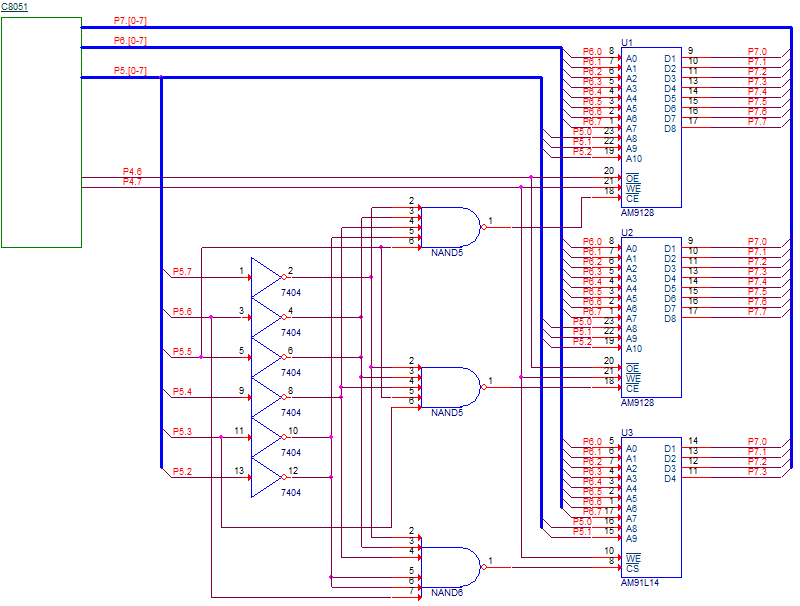
\includegraphics{schematic.png}
			\caption{Circuit schematic for part 3}
			\label{schematic}
		\end{figure} 
	\pagebreak
	\subsubsection{Code}
		\lstinputlisting{part3.c}
	
	
\section{References} 
\noindent
``MPS Lab 1," in RPI ECSE Department, 2016. [Online]. Available: \url{http://www.rpi.edu/dept/ecse/mps/MPS_Lab_Ex1-IDE_ANSI.pdf}. Accessed: Sep. 17, 2016.\\
\newline\noindent
``C8051 Manual," in RPI ECSE Department, 1.4 ed., 2005. [Online]. Available: \url{https://www.ecse.rpi.edu/courses/CStudio/Silabs/C8051F12x-13x.pdf}. Accessed: Sep. 17, 2016.








\end{document}